\documentclass{scrartcl}
\usepackage[utf8]{inputenc}
\usepackage{hyperref}
\usepackage{url}
\usepackage{graphicx}
\usepackage{float}
\usepackage{array}
\usepackage{booktabs}
\usepackage{tikz}
\usetikzlibrary{positioning, backgrounds, arrows.meta}
\usepackage{cleveref} % this must be the last package to be loaded

\newcommand{\emailaddr}[1]{\href{mailto:#1}{\texttt{#1}}}

\title{\LARGE
    Distributed Lupus in Fabula
}
\subtitle{Frontend \& Lobby --- Individual Contribution Report\\
    Final Report for the Distributed Systems Course --- A.Y. 2025/2026}

\author{
    Jacopo Bonifazi \\ \emailaddr{jacopo.bonifazi@studio.unibo.it}
}

\date{July 14, 2026}

\begin{document}

\maketitle


\section{Concept}\label{concept}

The project is a real-time, multiplayer, browser-based implementation of
the social deduction game \emph{Lupus in Fabula} (\emph{Werewolf}). From
the end-user standpoint, the product is a web application with a
graphical user interface (SPA, Single-Page Application): players open
the game in a browser on desktop or mobile and interact through a
graphical interface, without installing anything.

The use case is the following. A player creates a game room and shares a
short room code with friends; the others join the same room from their
own devices. Once at least the minimum number of players has joined and
declared themselves ready, the host starts the match. From that moment
the system drives a cyclic day/night state machine in which players
vote, and hidden roles (werewolf, seer, villager) perform their night
actions. Interaction is synchronous and short-lived: players interact
intensively for the whole duration of a match (a few minutes), several
times in a session, and every action must be reflected almost
immediately on every other player's screen.

Users are geographically distributed (each player on a different
machine and network), which is the first reason distribution is needed.
The second, and central for this course, is fault tolerance: since a
match is a shared, stateful, real-time session, the system must survive
transient client disconnections and the failure of a single server
instance without losing the game. The third reason is horizontal
scalability: multiple backend instances behind a load balancer must be
able to serve players of the same match even when those players are
connected to different instances. These three needs shape the whole
design.

\section{Requirements Elicitation and Analysis}\label{requirements}

\paragraph{Functional requirements (frontend/lobby scope).}
\begin{description}
  \item[F1] A user can create a room and obtain a shareable room code,
  or join an existing room by entering that code and a nickname.
  \emph{Acceptance: after creating/joining, the user reaches the lobby
  and appears in the players list on every connected client.}

  \item[F2] The lobby shows the list of connected players in real time,
  their ready status, and who the host is. \emph{Acceptance: when a
  player joins/leaves or toggles ready, all clients update the list
  without a page reload.}

  \item[F3] The host can configure the role setup (number of werewolves
  and seers) and start the match only when the start conditions are met
  (at least 5 ready players, at least 1 werewolf, and at least 1 plain
  villager remaining). \emph{Acceptance: the start control
  is disabled until the conditions hold, and starting transitions all
  clients to the game screen.}

  \item[F4] During the match the client displays the current phase
  (day/night), the alive/eliminated players, and a visual countdown for
  the current phase. \emph{Acceptance: on a phase change the UI updates
  on all clients and the countdown reflects the server-provided
  deadline.}

  \item[F5] The client exposes, for each phase and role, only the
  permitted actions (day vote, werewolf night target, seer
  investigation), and disables them otherwise. \emph{Acceptance: an
  action is accepted by the server only when issued by an eligible
  player in the correct phase.}

  \item[F6] Chat has restricted visibility: a global channel visible to
  everyone during the day, a werewolves-only channel at night, and a
  dead-players channel. \emph{Acceptance: a message on a restricted
  channel is rendered only by the clients entitled to see it.}

  \item[F7] At the end of the match the client shows the outcome
  (winning faction) and reveals every player's role. \emph{Acceptance:
  the result screen is consistent across all clients and reflects the
  final state.}

  \item[F8] The host can remove a player from the lobby, and can restart
  a finished match, returning every player to the lobby. \emph{Acceptance:
  a kicked player is disconnected and removed from the players list on
  every client; restarting clears the previous outcome and returns all
  clients to the lobby screen.}

\end{description}

\paragraph{Non-functional requirements (relevant to the client).}
\begin{description}
  \item[N1] Real-time responsiveness: state changes propagated by the
  server must be reflected in the UI with negligible delay.

  \item[N2] Client-side resilience: after a transient disconnection, the
  client must be able to reconnect and recover the exact current game
  state, rather than desynchronising or forcing a restart.

  \item[N3] Consistency across instances: two players of the same match
  connected to different backend instances must observe the same state.
  (This is guaranteed by the backend/infrastructure; the client
  requirement is to be instance-agnostic, i.e.\ to work identically
  regardless of the instance it is routed to.)
\end{description}

\paragraph{Implementation constraints (frontend).}
The frontend is built with Vue~3 and the Socket.IO client. These are
consequences of design (an event-driven, reactive UI over a
bidirectional real-time channel) rather than externally imposed
constraints, and are justified in \cref{implementation}.

\subsection{Relevant Distributed System Features}\label{ds-features}

Below, only the features on which the client has a role are discussed;
the others (e.g.\ server-side replication, monitoring) are covered by
the rest of the team.

\paragraph{Transparency.} Distribution transparency is a requirement: a
player must not perceive which backend instance is serving them, nor
that other players may be attached to a different instance. The client
is therefore designed to be stateless with respect to game logic and
instance-agnostic (\cref{architecture}). Reconnection and instance
re-routing must be as invisible as possible.

\paragraph{Fault tolerance.} Highly relevant. A dropped connection
(closed tab, network glitch) must not corrupt the shared match. On the
client this manifests as automatic reconnection and a state
resynchronisation step upon re-entry (\cref{fault-tolerance}).
Uninterrupted service for the surviving players is desired; momentary
data loss on a single client is acceptable because the authoritative
state lives server-side.

\paragraph{Scalability.} Relevant at the system level; the client
contributes by not assuming a single server and by working correctly
behind a load balancer.

\paragraph{Security / roles.} There is no sensitive personal data and no
cryptographic authentication; however there are multiple roles with
different visibility rights (werewolf vs.\ seer vs.\ villager, alive
vs.\ dead), which is an authorization concern discussed in
\cref{security}.

\paragraph{Not relevant.} Strong data durability, geographic
partitioning of data, and interoperability with external systems are
not requirements of this project.

\section{Design}\label{design}

\subsection{Architecture}\label{architecture}

The overall system follows an event-based architectural style layered
over a client/server organisation: clients and server exchange named
events over a persistent bidirectional channel, and the server
propagates events among its instances through a message broker. This
section describes the client side of that architecture.

The frontend is a Single-Page Application organised in three internal
layers:
\begin{itemize}
  \item \textbf{Views} (screens): they only present state and collect
  user input; they never talk to the network directly.
  \item \textbf{Stores} (application state): they hold the reactive
  client state, register the listeners for server events, and expose
  the actions that emit events to the server.
  \item \textbf{Communication layer} (a single Socket.IO wrapper): the
  only component that touches the network.
\end{itemize}

The guiding principle is that the client is event-driven and
\emph{stateless with respect to game logic}: it does not decide who
dies, when a phase ends, or who wins. It sends the user's intentions
(commands) to the server and reacts to the authoritative events the
server sends back, re-rendering accordingly. This choice directly serves
N2 and N3: because the client holds no authoritative state, it can
always be re-synchronised from the server after a fault and it behaves
identically regardless of the instance it is attached to.

\subsection{Infrastructure}\label{infrastructure}

From the infrastructure viewpoint the frontend is a client component. It
is served as static assets and, at runtime, opens a single long-lived
connection towards the backend. The client does not discover instances
by itself: it always targets a single stable endpoint (the reverse
proxy), and the proxy is responsible for routing the connection to one
of the backend instances. The endpoint is provided to the client at
build time through a configuration variable (\cref{deployment}), so the
same codebase works unchanged in the local, containerised, and
orchestrated environments.

\subsection{Modelling}\label{modelling}

\paragraph{Domain entities on the client.} The client mirrors a subset of
the domain: players (id, nickname, host flag, ready flag, alive flag,
and, once revealed, role), the room (code, role setup), the match
(phase, round, timer deadline, current votes, own role, outcome), and
chat messages (author, text, channel).

\paragraph{Mapping entities to components.} Consistently with the
``video-game'' mapping pattern, the authoritative state lives
server-side (in the shared store), while the client keeps only a local,
derived copy needed for rendering. This is why the client can be
discarded and rebuilt from a server snapshot at any time.

The client state is partitioned into three reactive stores, each with a
clear responsibility:
\begin{itemize}
  \item \textbf{Lobby store}: room code, players list, host, ready set,
  and role setup (number of werewolves/seers).
  \item \textbf{Game store}: the phase state machine
  (\textsc{lobby}\,$\rightarrow$\,\textsc{night}\,$\rightarrow$\,\textsc{day}\,$\rightarrow$\,\textsc{voting}\,$\rightarrow$\,\textsc{ended}),
  the player's own role, the phase timer, the vote tally, the pause
  state, and the final outcome.
  \item \textbf{Chat store}: the messages, the active channel, and the
  set of already-seen message identifiers used for de-duplication.
\end{itemize}

\paragraph{Domain events and message kinds.} The client exchanges two
kinds of messages with the server: \emph{commands} it emits (e.g.\ ``cast
a vote'', ``werewolf target'', ``toggle ready'', ``start game'') and
\emph{events} it receives describing facts that already happened (e.g.\
``phase changed'', ``role assigned'', ``player eliminated'', ``game
ended''). The full contract is given in \cref{interaction}. A REST
request/response query is also used once, to fetch the initial state
when entering the game screen.

\subsection{Interaction}\label{interaction}

Client and server communicate over a single persistent, bidirectional
channel using a publish/subscribe interaction pattern: the client
subscribes to named events and emits commands; the server, upon a
command, updates the authoritative state and broadcasts the resulting
event to all clients in the room, propagating it across instances
through the broker so that players on other instances receive it too.

The rule is strict and important for consistency: the client never
assumes its command succeeded until it receives the corresponding
confirmation event from the server. For example, casting a vote does not
update the local tally directly; the tally is updated only when the
server broadcasts the vote update.

\Cref{tab:events} summarises the event contract (the exact names shared
with the backend).

\begin{table}[H]
  \centering
  \small
  \begin{tabular}{@{}p{2.0cm}p{6.0cm}p{5.2cm}@{}}
    \toprule
    \textbf{Scope} & \textbf{Received (server $\to$ client)} & \textbf{Emitted (client $\to$ server)} \\
    \midrule
    Lobby &
      \texttt{game\_state\_sync}, \texttt{player\_joined}, \texttt{player\_left}, \texttt{player\_ready}, \texttt{role\_setup\_updated}, \texttt{room\_closed}, \texttt{kicked} &
      \texttt{lobby:player\_ready}, \texttt{lobby:update\_settings}, \texttt{lobby:start\_game}, \texttt{kick\_player} \\
    \addlinespace
    Game &
      \texttt{game\_start} / \texttt{start\_game}, \texttt{phase\_changed}, \texttt{role\_assigned}, \texttt{vote\_update}, \texttt{player\_eliminated}, \texttt{player\_killed}, \texttt{seer\_result}, \texttt{no\_elimination}, \texttt{game\_ended}, \texttt{game\_paused}, \texttt{game\_resumed} &
      \texttt{cast\_vote}, \texttt{wolf\_vote}, \texttt{seer\_action}, \texttt{return\_to\_lobby} \\
    \addlinespace
    Chat &
      \texttt{chat\_message} &
      \texttt{chat\_message} \\
    \bottomrule
  \end{tabular}
  \caption{Socket.IO event contract between client and server.}
  \label{tab:events}
\end{table}

As an end-to-end example, a day vote unfolds as: (1) the player selects
a target in the UI; (2) the game store performs a local eligibility
check (alive, correct phase, not self) and emits \texttt{cast\_vote};
(3) the server records the vote in the shared state and broadcasts
\texttt{vote\_update}; (4) all instances forward the event; (5) every
client's game store updates its tally and the UI shows the new votes.
The initiating client itself only ``sees'' its vote once the broadcast
returns, which keeps all clients consistent (\cref{fig:client-internal-vote}).

\begin{figure}[H]
  \centering
  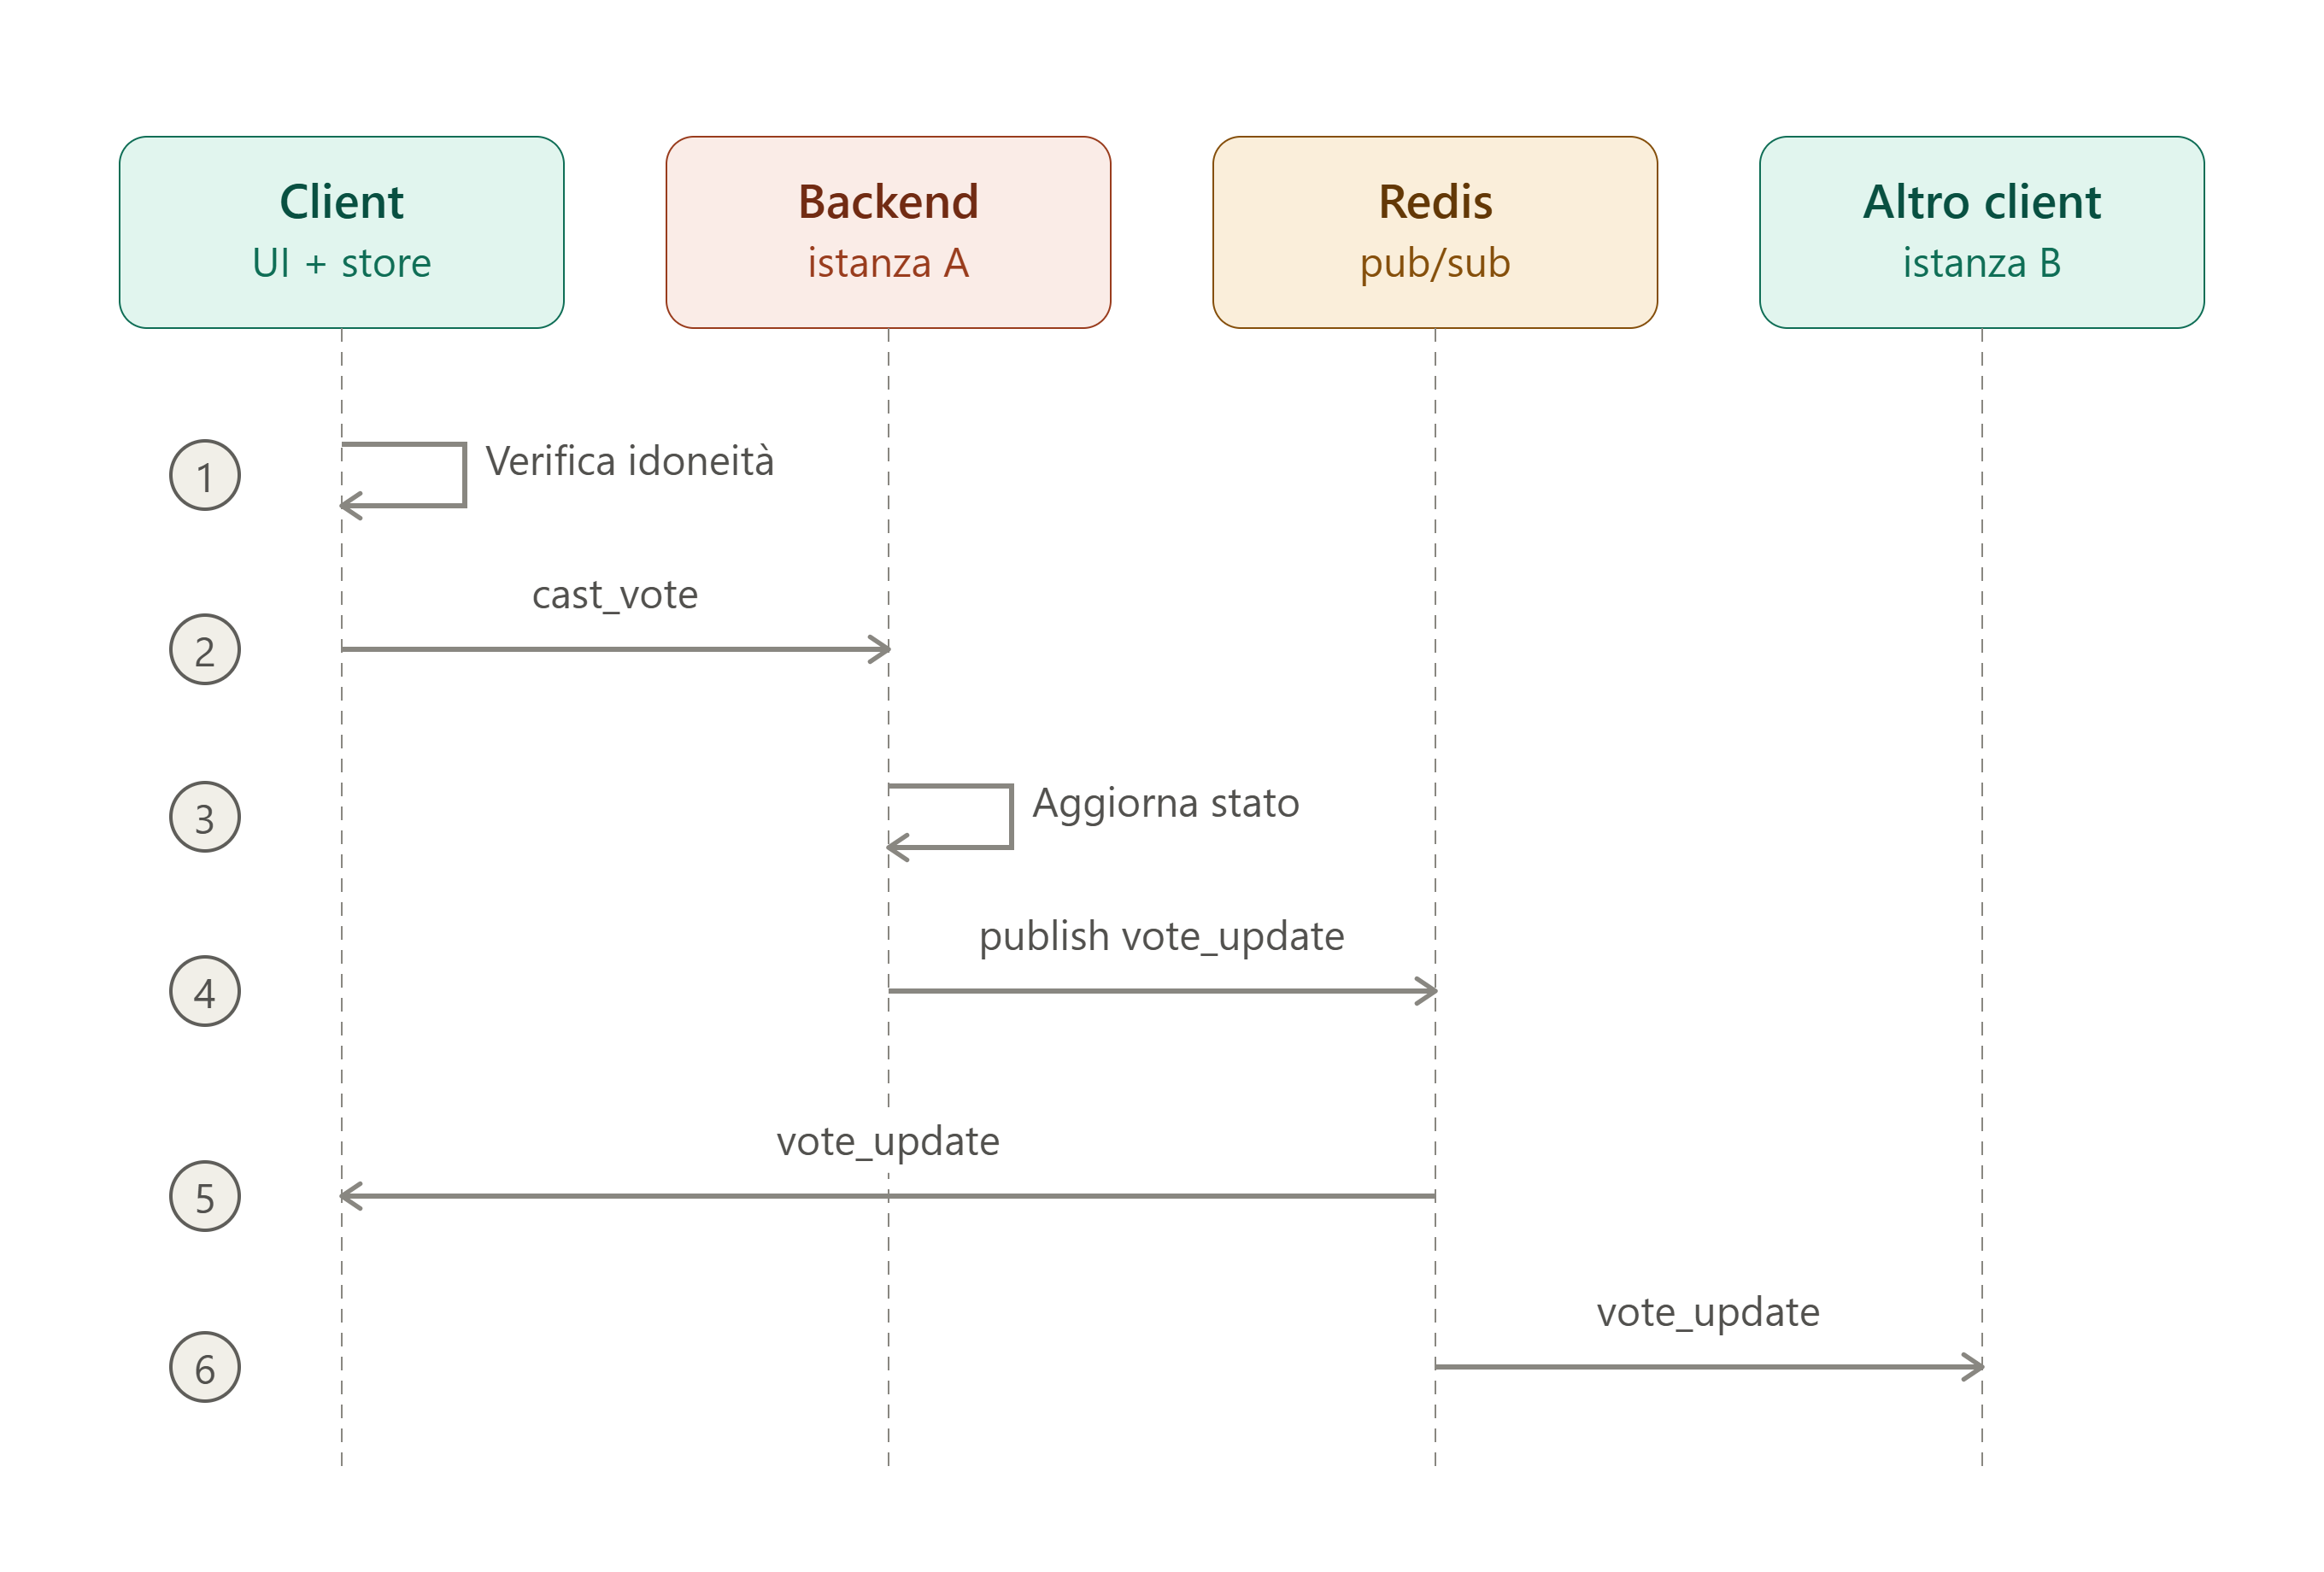
\includegraphics[width=0.9\textwidth]{figures/sequence_diagram_vote.png}
  \caption{Client-internal path of the day-vote example above, zooming
    into a single client. The local check is optimistic UI feedback
    only, not an authoritative decision: the vote is not considered cast
    until \texttt{vote\_update} returns from the server and the store
    updates its reactive tally, which is exactly what the view
    re-renders from --- no client component ever writes authoritative
    game state (\cref{behaviour}).}
  \label{fig:client-internal-vote}
\end{figure}

\subsection{Behaviour}\label{behaviour}

The client's components split cleanly into stateful and stateless.

The \textbf{stores are stateful}: each one registers its listeners once,
and on every incoming event it updates the reactive state. For instance,
on \texttt{phase\_changed} the game store updates the phase and the
timer deadline; on \texttt{role\_assigned} it stores the player's own
role; on \texttt{vote\_update} it refreshes the vote tally; on
\texttt{player\_eliminated}/\texttt{player\_killed} it marks a player as
dead; on \texttt{game\_ended} it records the outcome.

\Cref{fig:phase-fsm} visualises the phase state machine that the game
store tracks this way: every transition shown is driven by an incoming
\texttt{phase\_changed} or \texttt{game\_ended} event, never decided by
the client itself.

\begin{figure}[H]
  \centering
  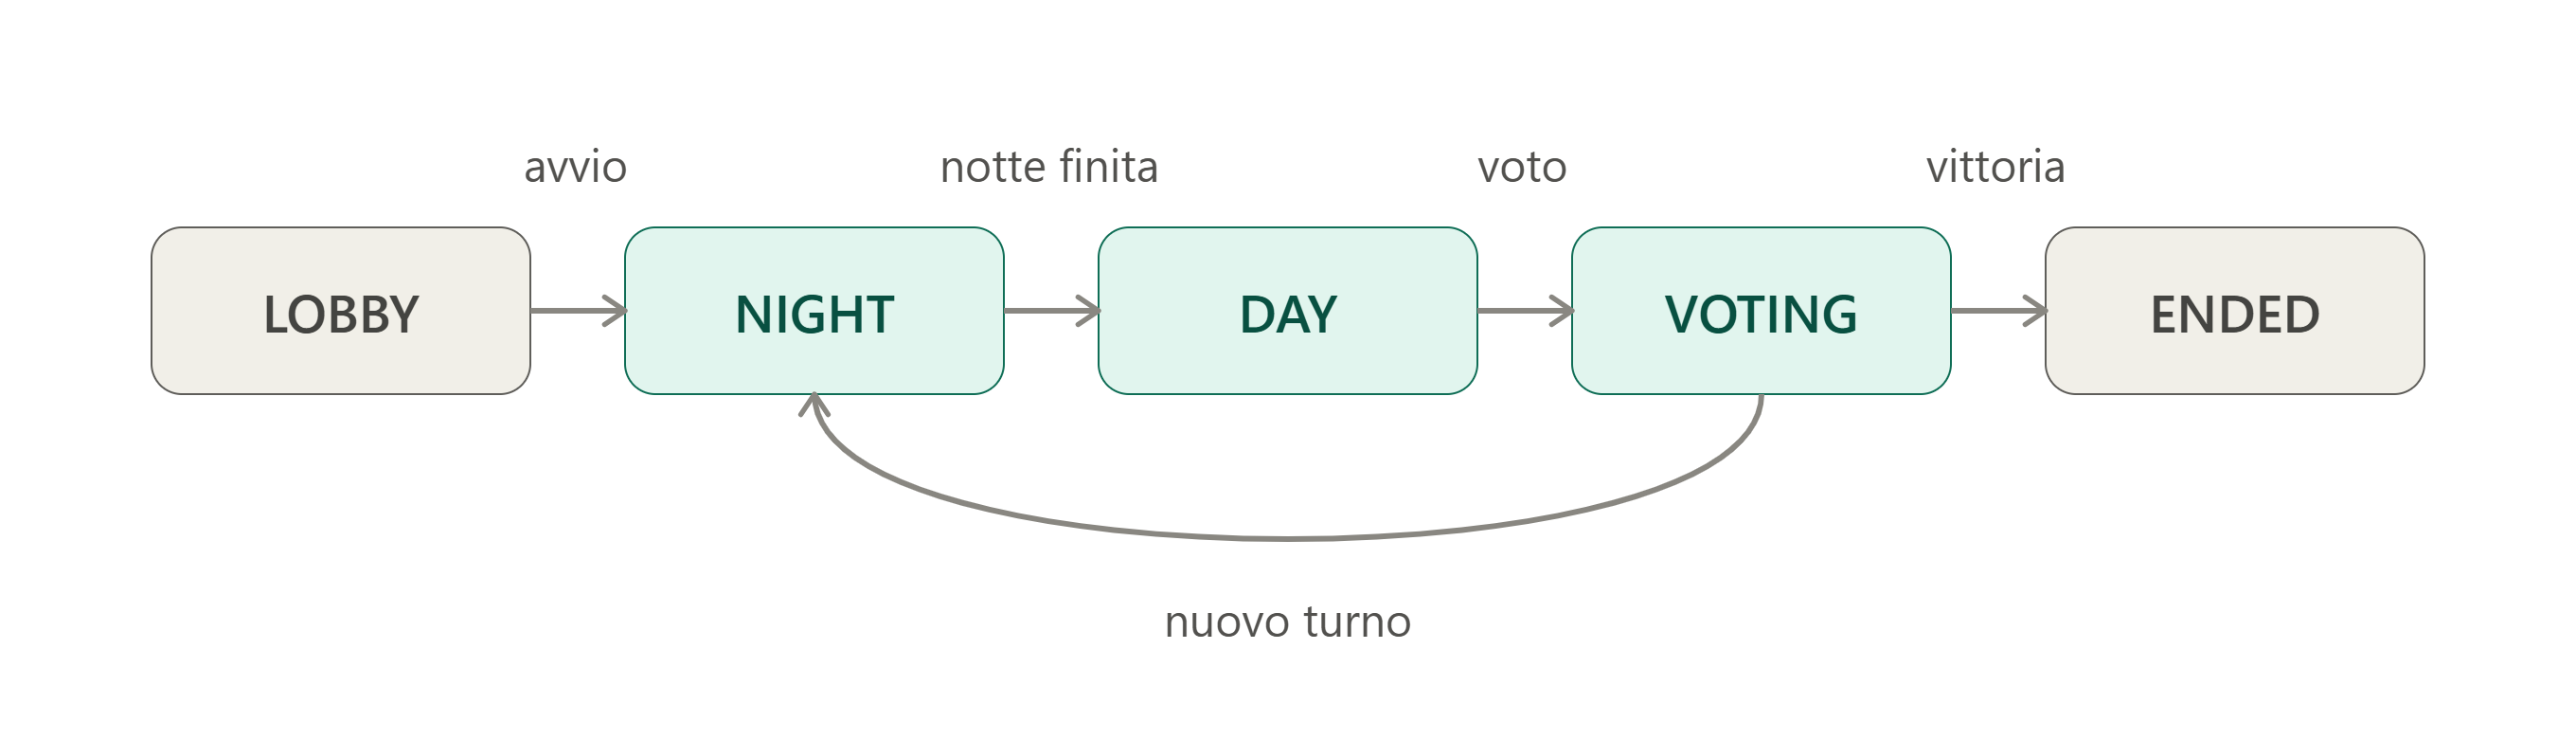
\includegraphics[width=0.9\textwidth]{figures/state_diagram_game_phase_client.png}
  \caption{Client-side view of the phase state machine, as tracked by
    the game store (\cref{modelling}). The client only ever renders the
    phase the server last announced.}
  \label{fig:phase-fsm}
\end{figure}

The \textbf{views and visual components are effectively stateless}: they
read the reactive state and re-render automatically thanks to the
framework's reactivity. They do not hold authoritative data; a screen is
just a function of the current store state.

Crucially, \textbf{no client component updates the authoritative game
state}. The client only proposes commands; the server is the sole
component in charge of updating the system state and then notifying
everyone. This clean separation is what makes client resynchronisation
(\cref{fault-tolerance}) safe.

\subsection{Data and Consistency Issues}\label{data-and-consistency-issues}

The client persists no authoritative data: its state is kept in memory
only, for the lifetime of the session, and is always reconstructable
from a server snapshot. A small piece of identity information (the
player's client identifier and the room code) is kept in the browser
session storage so that a page reload can re-attach to the same match.

Two consistency concerns are handled on the client side. First, because
the initiating client waits for the server broadcast before updating
(\cref{interaction}), all clients converge on the same tally/phase/outcome.
Second, in a multi-instance deployment the same event may reach a client
more than once (e.g.\ a chat message forwarded through the broker); the
chat store therefore de-duplicates messages by tracking already-seen
message identifiers, so a duplicated delivery is rendered only once.
This is a concrete, client-side accommodation of the underlying
distributed, at-least-once delivery.

\subsection{Fault-Tolerance}\label{fault-tolerance}

On the client, fault tolerance rests on three mechanisms.

\paragraph{Automatic reconnection.} The communication layer is
configured to retry the connection automatically after a drop (a
bounded number of attempts with a fixed delay). A transient network
glitch is therefore recovered without user intervention.

\paragraph{State resynchronisation on re-entry.} Because the
authoritative state lives server-side, when the client reconnects (or
when a paused match resumes) the server sends a full snapshot event that
the client applies wholesale, realigning its stores to the exact current
state. The client thus never tries to ``guess'' what it missed while
disconnected; it simply adopts the server truth.

\paragraph{Pause feedback.} When the server signals that the match has
been paused (e.g.\ while waiting for a disconnected player to return),
the client shows a pause banner; when the server signals resume, the
banner is cleared and play continues. The authoritative decision to
pause/resume and to freeze the phase timer is taken server-side; the
client only reflects it.

The design principle behind all three is the same: the client is
disposable and can always realign to the server. This satisfies N2 and
keeps the surviving players' experience uninterrupted.

\subsection{Availability}\label{availability}

The client does not implement caching or load balancing (those belong to
the infrastructure). Its contribution to availability is behavioural:
under a network partition the client does not fail hard; it enters a
reconnecting state, informs the user, and keeps retrying, then
resynchronises once connectivity is restored. Because the client is
instance-agnostic, when the load balancer re-routes a reconnection to a
different backend instance the client recovers the same match state
through the snapshot mechanism.

\subsection{Security}\label{security}

The system does not process sensitive personal data and does not employ
cryptographic authentication or encryption of application messages; this
is a deliberate scope decision for a casual, ephemeral party game.

\paragraph{Identification.} On connection the client presents an
identifier (the chosen nickname acting as client id) and the room code;
the server uses these to attach the socket to the correct room and
player. A server-side check prevents an active duplicate identity within
the same room.

\paragraph{Authorization by role and state.} The meaningful
access-control concern is visibility, and it is enforced on both sides.
The client renders only the information a player is entitled to see:
chat channels are filtered by role/liveness (global for everyone,
werewolves-only at night, dead-only), and the action controls are
enabled only for the eligible role in the correct phase. This
client-side filtering is a UX safeguard; the authoritative enforcement
of who may perform which action is done by the server.

\section{Implementation}\label{implementation}

\paragraph{Network protocol and data representation.} Client/server
communication uses WebSocket as the transport, accessed through the
Socket.IO client library, which provides the event abstraction and
automatic reconnection on top of it. The transport is explicitly
restricted to WebSocket (the HTTP long-polling fallback is disabled) to
keep a single, clean upgrade path behind the reverse proxy. In-transit
messages are represented as JSON event payloads. A single REST endpoint
(over HTTP) is used to fetch the initial game state when entering the
game screen; every other interaction is event-based.

\paragraph{Authentication/authorization.} As discussed in
\cref{security}, there is no token-based authentication; identity is a
nickname-based client id passed in the connection handshake, and
authorization is expressed as role/phase-based visibility rather than as
a permission system.

\subsection{Technological details}\label{technological-details}

The frontend is implemented with \textbf{Vue~3} (Composition API,
\texttt{<script setup>}), built and served in development by
\textbf{Vite}, with \textbf{Vue Router} for client-side routing and
\textbf{Pinia} for state management; real-time communication uses the
\textbf{socket.io-client} library.

\paragraph{Routing.} Four routes map to the four screens: home
(\texttt{/}), lobby, game, and results, the last three optionally
parameterised by room id.

\paragraph{State stores (Pinia).} Three stores implement the model of
\cref{modelling}: a lobby store, a game store, and a chat store. Each
store exposes reactive state, computed selectors (e.g.\ alive players,
own role, whether an action is currently allowed, the visible chat
messages), the event listeners, and the command-emitting actions.

\paragraph{Communication layer.} A single Socket.IO connection is shared
across the whole application (one module-level instance rather than one
per component). Its notable design points are: the WebSocket-only
transport; an authentication payload carrying the client id and room id,
consumed by the server's connection handler; automatic reconnection with
a bounded number of attempts; and a pending-listener registry that lets
stores register event handlers before the socket actually exists and
re-binds them when the connection opens (this avoids race conditions
between component mount and connection). Listeners are
de-registered/re-registered around reconnections to avoid duplicate
handlers, which, combined with message de-duplication, prevents
duplicated or lost chat messages.

\paragraph{Reusable components.} The UI is composed of small components:
a player card (rendered as an SVG with a hidden back or a revealed
role), an avatar (deterministic colour and initials from the player id),
a chat box, a circular phase timer (whose colour changes as the deadline
approaches), a role-icon component, and an info box. Views compose these
components and bind them to the stores.

\section{Validation}\label{validation}

\subsection{Automatic Testing}\label{automatic-testing}

The frontend is unit-tested with \textbf{Vitest} and the Vue testing
utilities. The tests focus on the parts that carry logic rather than
presentation, i.e.\ the stores and the routing:

\begin{itemize}
  \item \emph{Store tests} verify how the stores react to incoming
  events (for example that a phase-change event updates the phase, that
  a vote update updates the tally, and that chat de-duplication discards
  an already-seen message). Rationale: the stores encode the client's
  reaction to the event contract, which is the most defect-prone part of
  the client; they map onto the functional requirements F2--F8.

  \item \emph{Composable/router tests} verify auxiliary logic (e.g.\ the
  phase timer countdown and the route configuration).
\end{itemize}

Tests are run from the frontend project with the Vitest runner
(\texttt{npm run test:unit}).

The views are intentionally not unit-tested at the component level:
their behaviour is essentially a projection of the store state (already
tested) and is better validated end-to-end (below).

\subsection{Acceptance test}\label{acceptance-test}

End-to-end behaviour was validated manually, because it involves several
real clients interacting over the network in real time, which is
expensive to automate meaningfully. The main flows were exercised with
multiple browser windows in separate incognito sessions (to obtain
independent client identities): create room $\to$ join with several
players $\to$ ready/start $\to$ play through the day/night cycle $\to$
reach the result screen. Corner cases were tested explicitly, notably
transient disconnection and reconnection during a match (verifying state
resynchronisation), and the multi-instance scenario, where players of
the same room are deliberately spread across two backend instances to
confirm that events propagate to everyone and that the client behaves
identically regardless of the instance it is routed to.

\section{Deployment}\label{deployment}

The frontend is packaged with a multi-stage Docker build: a first stage
builds the static assets with Node, and a second stage serves them with
a static web server, exposing only the built bundle. The endpoint of the
backend used by the client is injected at build time through an
environment variable, so the same image works locally and in the
containerised/orchestrated deployment; at run time the client always
talks to the reverse proxy, which routes to a backend instance.

\paragraph{Note on the endpoint variable.} Since this variable is baked
into the bundle at build time, changing it requires rebuilding the
frontend image (not merely restarting the container). Its value must
match the path used by the proxy to route the real-time connection.

\section{User Guide}\label{user-guide}

\begin{enumerate}
  \item \textbf{Home.} On the landing screen, choose \emph{Create room}
  or \emph{Join room}. Creating produces a shareable room code; joining
  requires the code and a nickname (3--15 characters).

  \item \textbf{Lobby.} Share the room code with the other players.
  Everyone sees the live list of connected players and their ready
  state. Players toggle ready; the host can adjust the role setup and
  starts the match once at least 5 players are ready.

  \item \textbf{Game.} The screen shows the current phase (day/night),
  the alive and eliminated players, and a countdown. During the day
  players discuss and vote; at night the werewolves choose a target and
  the seer investigates. Only the actions allowed for the player's role
  and the current phase are enabled. Chat visibility follows the current
  channel (global by day, werewolves at night, dead players separately).

  \item \textbf{Results.} At the end the winning faction is announced
  and all roles are revealed. The host may restart the room (``play
  again''), which sends the other players back to the lobby.
\end{enumerate}

\section{Self-evaluation}\label{self-evaluation}

\subsection{Jacopo Bonifazi - Frontend \& Lobby}

My role in the group was to design and implement the entire frontend and
the lobby system: the user interface (home, lobby, game, and results
screens), the client-side state management with three Pinia stores, the
integration with the real-time channel via the Socket.IO client, and the
client-side handling of disconnection and recovery. I also owned the
definition of the Socket.IO event contract on the client side, in
coordination with the backend.

\paragraph{Strengths of the product.} The client is cleanly layered and
event-driven, which keeps game logic entirely on the server and makes
the UI a pure projection of the authoritative state; this made the
resynchronisation after a fault straightforward and robust
(\cref{fig:phase-fsm,fig:client-internal-vote}). The restricted-visibility
chat and the per-role, per-phase action gating meet the functional
requirements, and the message de-duplication correctly handles the
at-least-once delivery that arises in the multi-instance deployment.

\paragraph{Weaknesses / limitations.} The pause/resume experience
depends on server-side events that were still being finalised, so its
full behaviour was not completely exercised. The component-level UI is
validated mostly by manual end-to-end testing rather than automated
component tests. Some auxiliary REST scaffolding remained unused once
the interaction consolidated on the event channel.

\paragraph{Contribution.} Objectively, I delivered the full frontend and
lobby as planned, and additionally helped diagnose several integration
issues that surfaced in the containerised, multi-instance environment
(e.g.\ the WebSocket endpoint mismatch and the instance-local player
counting), which, although resolved server-side/infrastructure-side,
were identified from the client behaviour.

\section{Future works}\label{future-works}

From the client side, natural extensions are: completing the
pause/resume UX once the corresponding server events are finalised
(including a graceful ``player did not return'' outcome); adding
automated component/end-to-end tests to cover the UI flows that are
currently checked manually; removing the unused REST scaffolding now
that interaction is event-based; and small UX refinements such as
richer, always-legible error feedback on the entry screen.

\end{document}
